\chapter{新闻事件的可视化方法设计}
在第2章中我们已经介绍了一些文本可视化的方法,它们对于理解文本信息有着非常重要的作用。特别是对于时序文本的可视化,越来越多的新闻工作者,政府部门,社会工作者和科学研究人员表现出了极大的兴趣,他们希望能够通过直观的视觉图形中了解事件或故事随着事件的演化。
\section{Storyline 方法研究}
Storyline 是指描述的是人物之间随时间变化的社交关系,它将这些复杂的信息在一张图形上展现出来。该方法是受 Mounroe 发布在著名漫画网站 XKCD 的 "Movie Narrative Charts" \cite{xkcd657} 的启发。在这个连载漫画中,手绘的 Storyline 用于概括电影中角色之间的互动(如 Figure.\ref{xkcd} 所示)。
% BEGIN == XKCD 手绘图
\begin{figure}[!htb]
	\centering
		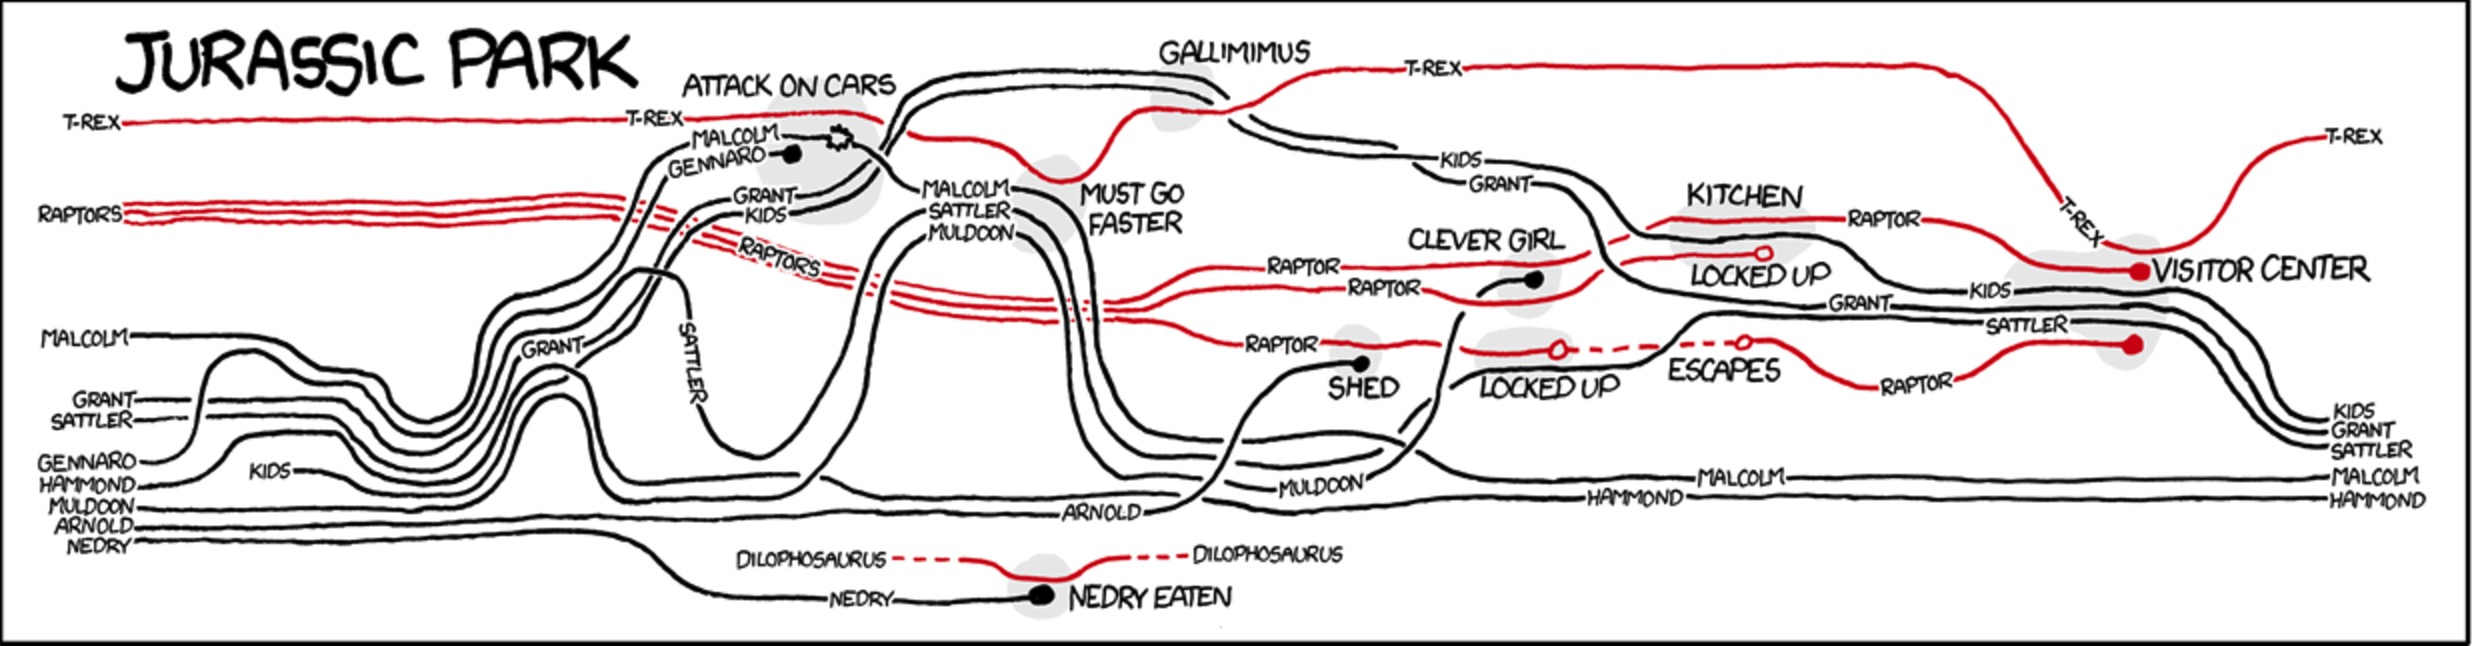
\includegraphics[width=\textwidth]{xkcd_jurassic_park}
	\caption{Jurassic park 人物关系叙事图,X轴表示时间,每个线条分别代表一个角色}
	\label{xkcd}
\end{figure}
% END == XKCD 手绘图
相比其它时间轴相关的可视化方法,storyline 通过线条来表示故事中的实体,并且通过与实体关联的线条的之间的距离变化来表示实体之间的关联关系。基于这样的基本思想,在不同的应用中已有一些特定的方法被提出,例如:TimeNets\cite{Kim:2010:TGD}用于从生育数据中跟踪世代关系,\cite{Reda2011}用于从动态的社交网络中跟踪社团的发展。然而这些方法都是针对特定问题提出的,通用性不强。PlotWeaver\footnote{http://ogievetsky.com/PlotWeaver/} 是一个在线的 storyline 编辑工具,它提供了友好的用户操作界面,可以让用户轻松的自己创建storyline。然而对于大规模文档集合,通过纯手工的方式创建storyline显然是一件耗时耗力的工作。Ogawa 和 Ma \cite{Ogawa:2010} 基于创建 storyline 的基本原则设计了一套能够自动生成 storyline 的启发式算法,不过用该方法创建的 storyline 相对比较简单,远不能跟由专业的艺术家手动绘制的结果相比。在此基础上Tanahashi 和 Ma\cite{tanahashi2012design} 提出了一套更加完成的方法框架,它将 storyline 的布局问题形式化为一个优化问题,并通过遗传算法进行求解。然而遗传算法需要花费相当长的时间才能得到理想的结果,同时也不支持交互式的调整。因此本文基于已有的研究成果,提出了一套方法框架,能够在较短的时间内生成同样效果的 storyline,并且提供一些交互式操作来优化和调整最终的可视化效果。

\subsection{设计原则}
在介绍 storyline 的设计准则之前,我们首先定义 storyline 中最基本的一对映射关系:
\begin{itemize}
\item \textbf{角色(Character 或 Entity)}
\item \textbf{线条(Thread)}
\end{itemize}
\textbf{Character} 是指故事中出现的人物或其他个体。新闻语料中,角色可以是人物、组织机构、国家等命名实体,它们一起构成了新闻故事六要素(时间、地点、人物、起因、经过和结果)之一的人物。电影、小说和新闻事件等通常都会有一个\textbf{主角(Leading Character)} 和若干的\textbf{配角(Ordinary Character)},所有的故事都围绕着主角展开和发展,并通过配角来充实整个故事。为了将故事中的 \textbf{Characters} 以及它们之间发生的事件映射到 storyline 中,便得到了 storyline 设计的基本原则:
\begin{itemize}
\item 水平轴上从左往右的\textbf{线条}表示故事中一个\textbf{角色}完整的生命周期。
\item 多个 \textbf{线条} 在某一时间段聚拢到一块,表示有这些\textbf{角色}共同参与了一个事件。线条之间的\textbf{收敛}和\textbf{发散}分别表示角色间的事件的开始和结束。
\end{itemize}
\textbf{Thread} 作为 \textbf{Characters} 的载体,每一个 \textbf{Thread}  都可以看作是故事的维度,一个由 \textbf{Threads} 组成的集合以及它们之间的位置随时间的变化(如:\textbf{收敛 Convergence},\textbf{发散 Divergence} 和\textbf{交叉 Intersection})描述了整个故事的发展变化。以上设计原则可以指导我们设计出更美观且易于理解的图形,因此被许多研究者广泛采用\cite{Ogawa:2010, Kim:2010},并在构建特定领域的 storyline 上获得了一定程度上的成功。然而,这些以上原则并没有很好的将文本的上下文信息(如,位置)表现出来。为了更好的描述事件发生的位置信息,Tanahashi 和 Ma \cite{tanahashi2012design} 在storyline 中用一个封闭的轮廓线作为背景将事件圈起来,并用不同的颜色表示不同的事件。同时为了让 storyline 展现得更加美观并增强可读性,Tanahashi 和 Ma 还添加了一条新的标准:
\begin{itemize}
\item 线条只有在收敛和发散的时候才可以偏离原始的方向。
\end{itemize}
也就是说,要尽可能让线条保持直线,减少线条的摆动。本文中,我们将采用以上这些原则来设计我们的 storyline。

\subsection{最优化度量}
\label{metrics}
给定一个角色(实体,人物)的集合以及它们之间在时间上的关联关系,我们的目标是要构建出一个美观且易于理解的 storyline 可视化图形。图形布局的构建可以分解为一系列的最优化求解问题,在我们的布局最优化方法中,我们采用 Tanahashi 和 Ma \cite{tanahashi2012design} 提出的最优化度量标准来定义我们的优化目标。
\begin{itemize}
\item \textbf{线条交叉 Line Crossovers}:最小化线条交叉的数量。
\item \textbf{线条摆动 Line Wiggles}:增强线条的笔直和连续性。
\item \textbf{空白距离 White Space Gaps}:最小化空白空间之间的距离,增强紧凑度。
\end{itemize}
很显然\textbf{线条交叉}容易造成图形的混乱,所以应该最小化交叉的数量。\textbf{线条摆动}是指线条偏离了原始的方向,这会打断线条的连续性,因此减少线条摆动次数可以增强可读性。\textbf{空白距离}是指图形中两个可视元素之间的空白空间的大小,空白空间是图形中区分元素的必要组成部分,然后过度的距离不仅容易造成空间的浪费,更重要的是容易让读者误以为这是上下文中角色之间的语意距离,所以也应当减少不必要的空白空间。

\section{Storyline 数据定义}
在 Storyline 的可视化中用到的数据最基本的形式就是各个角色之间按时间先后顺序排列的交互列表。这些角色之间的一系列交互可以被拆分成一系列\textbf{会话 Session},每个\textbf{会话}代表了一个时间跨度以及这段时间内有交互的角色集合。严格意义上,我们可以将\textbf{会话}定义为包含以下元素的基本单元:
\begin{itemize}
\item \textbf{起始时间}
\item \textbf{时间跨度}
\item \textbf{成员列表}
\end{itemize}
\textbf{起始时间}表示\textbf{会话}从何时开始,\textbf{时间跨度}表示该\textbf{会话}的持续时间,\textbf{成员列表}是指参与本次\textbf{会话}的所有角色的集合。 Listing \ref{list:json-sample} 是用Json格式封装以上数据的一个简单样例。
% BEGIN == JSON Schema & Example
\begin{listing}
% 设置行间距和段间距
\linespread{0.9}
\begin{minted}[frame=single, tabsize=4]{js}
{
    "sessions": [
        {
            "id": 0,
            "start": 0,
            "duration": 5,
            "characters": [
                0,
                2
            ]
        }
        {
            "id": 1,
            "start": 5,
            "duration": 10,
            "characters": [
                0,
                3,
                10
            ]
        }
   ]
}
\end{minted}
\caption{Storyline输入数据格式(Json)} 
\label{list:json-sample}
\end{listing}
% END == JSON Schema & Example

\subsection{可视化元素定义}
在 storyline 中可视化元素包括: \textbf{线条},\textbf{角色标签},\textbf{节点}和\textbf{会话框}。针对每一个可视化元素,他们分别包含了多种呈现方式。
\begin{itemize}
\item \textbf{线条}。颜色,为了便于区分不同角色,每个线条的颜色必须与和它相邻的线条不同,最好的情况时保证所有线条的颜色均不相同;宽度,所有线条的宽度都一样。
\item \textbf{角色标签}。为了便于理解不同线条所代表的角色,角色标签将出现在线条的起点和终点。
\item \textbf{节点}。线条中空心圆点表示角色的出现,实心圆点表示角色的消失。
\item \textbf{会话框}。会话框呈现不规则的封闭图形,会话框需要将参与会话的线条都囊括在内,同时必须排除未参加该会话的线条。
\end{itemize}

\section{Storyline 布局算法}
本章节我们主要介绍 storyline 布局设计中的一些思想和使用的相关算法。首先我们需要对这个实际问题进行形式化的描述,也就是将它表述成了数学问题,然后用数学公式进行定义。
\subsection{问题定义}
\label{section:problem-definition}
 从数学角度考虑,Storyline 的布局可以看成是一个有层次关系的 DAG(Directed Acyclic Graph)图。如 Figure \ref{fig:construct-1} 中的每个节点代表了一个会话,不同颜色的有向边代表了不同角色的信息流。其中,会话在水平方向的位置与其发生的时间相关,越早发生则在水平方向上越靠左边;会话的垂直位置没有具体的含义,仅仅是为了更好的布局而确定的。在确定了 Storyline 的 DAG 图之后,第二步要做的就是将会每个会话的内部信息表示出来。如 Figure \ref{fig:construct-2} 所示,图中的每个虚线框与 Figure \ref{fig:construct-1} 中的节点对应,参与该会话的会话的每个角色在在会话内部分别有一个线段表示,进入会话时,线段会聚,离开会话时,线段发散,从而保证在会话内线段之间的间距较小。
% BEGIN == Construct
\begin{figure}[htb]
	\centering
	\subfigure[DAG 图构建]{
		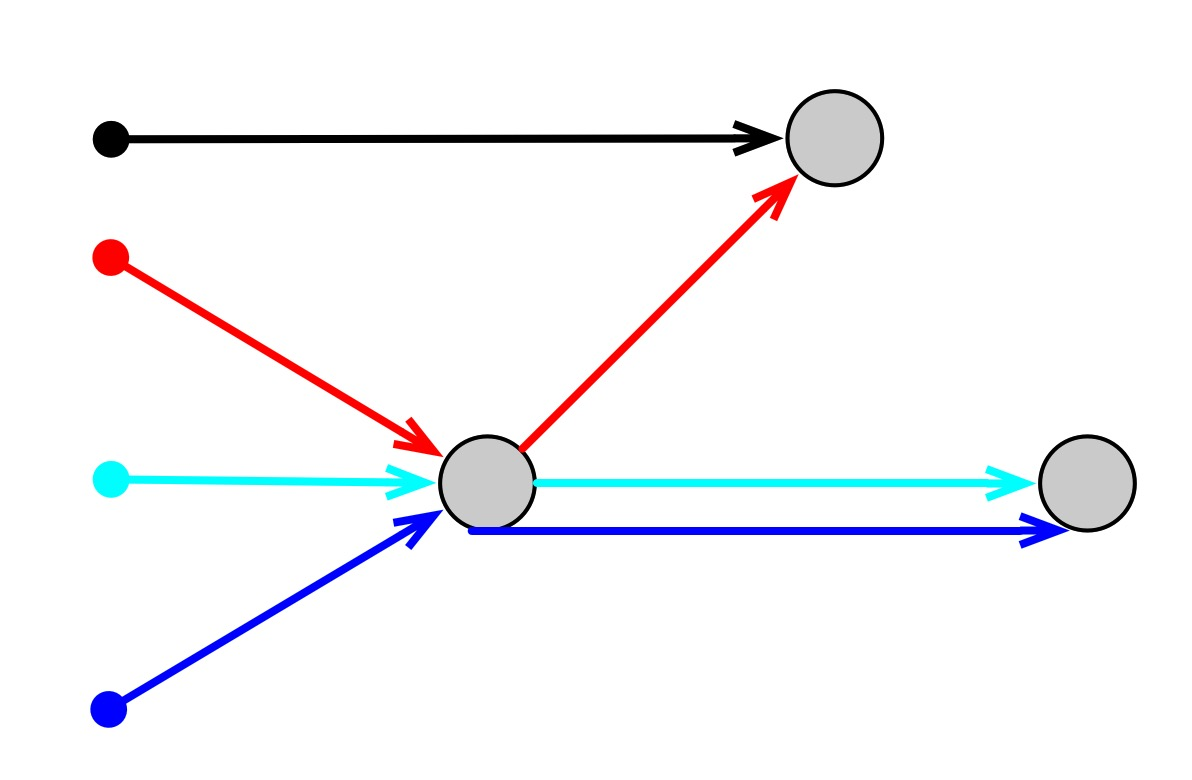
\includegraphics[width=0.4\textwidth, fbox]{construct-1}
		\label{fig:construct-1}
	}
	\subfigure[会话位置确定,线条排序]{
		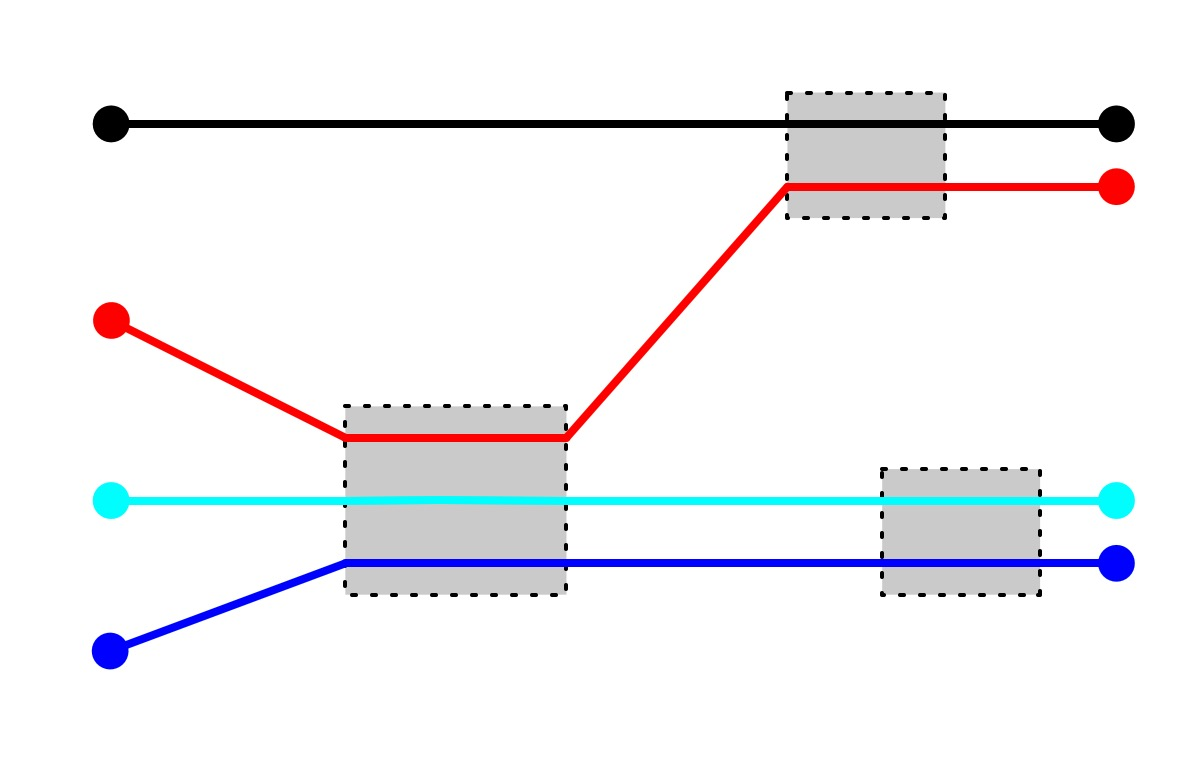
\includegraphics[width=0.4\textwidth, fbox]{construct-2}
		\label{fig:construct-2}
	}
	\caption{Stroyline 布局方法}
	\label{fig:storyline-dag}
\end{figure}
% BEGIN == Construct

布局设计中我们的主要目标就是最小化 \ref{metrics} 小节中提出的三个度量指标:\textbf{Line Crossover number},\textbf{wiggle number},\textbf{white space gaps}。 显然这是一个解空间极大的优化问题,要设计一个方法能够同时最优化以上三个指标是一项很困难的任务。对于此类解空间太大而不能轻易求得全局最优解的问题,我们也可以采用\textbf{遗传算法}\cite{tanahashi2012design} 等启发式算法来求得一个接近最优的解决方案。然而,遗传算法的不足是获得的局部最优解经常会比较差,并且容易造成早熟收敛的问题。

既然一步到位同时优化以上三个指标比较困难,很自然的就想到将其分解成几个独立的子问题。每个子问题分别最优化 \ref{metrics} 小节中的一个度量指标。子问题处理的原则是重要指标优先处理,因为它们对最终的可视化效果影响最为严重,更重要的是,在优化后续指标时不能影响前一指标的效果。显然线条交叉对结果的影响,减少线条的摆动以及空白距离次之。基于此,我们将问题分解成以下三个步骤,如 Figure \ref{fig:layout-steps} 所示:
% BEGIN == Framework
\begin{figure}[htb]
	\centering
	\subfigure[初始布局]{
		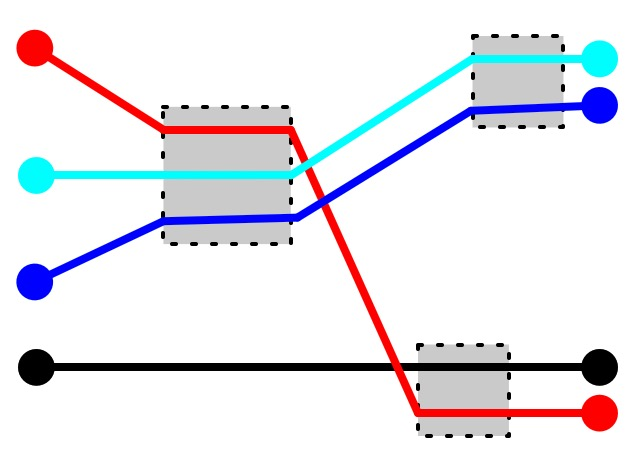
\includegraphics[width=0.2\textwidth, fbox]{framework-1}
		\label{fig:layout-step-1}
	}
	\subfigure[排序]{
		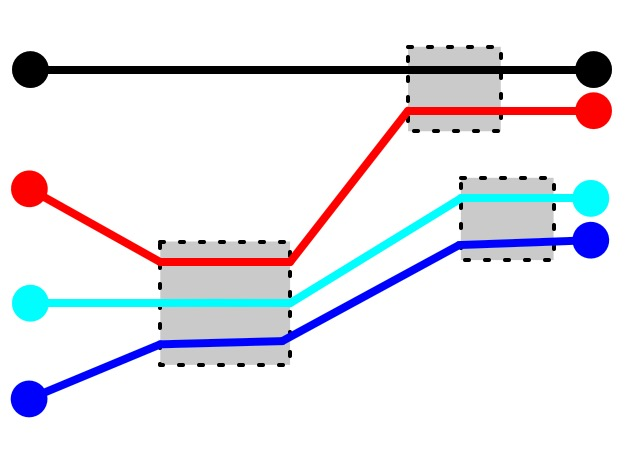
\includegraphics[width=0.2\textwidth, fbox]{framework-2}
		\label{fig:layout-step-2}
	}
	\subfigure[对齐]{
		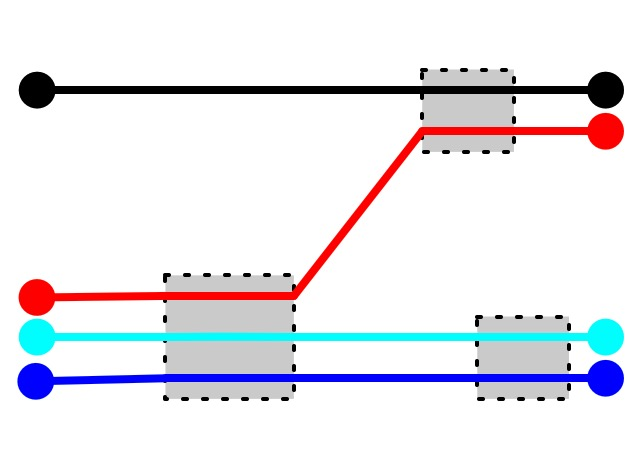
\includegraphics[width=0.2\textwidth, fbox]{framework-3}
		\label{fig:layout-step-3}
	}
	\subfigure[压缩]{
		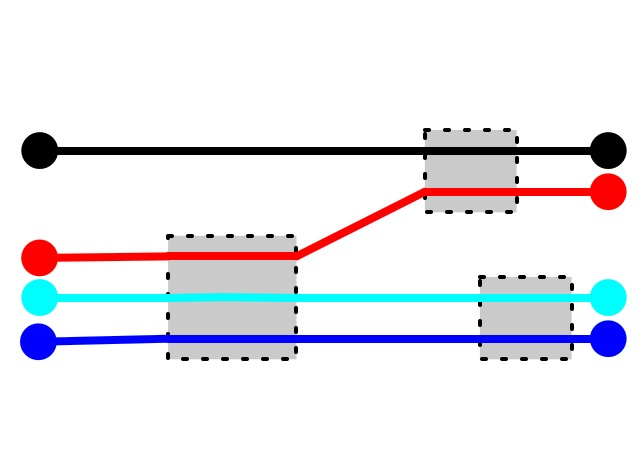
\includegraphics[width=0.2\textwidth, fbox]{framework-4}
		\label{fig:layout-step-4}
	}
	\caption{布局算法的整体框架}
	\label{fig:layout-steps}
\end{figure}
% BEGIN == Framework

\begin{itemize}
\item \textbf{步骤1:排序。}影响线条交叉数目最直接的因素就是线条的排列顺序,而影响线条排序最重要的因素就是会话的位置,因此为了减少线条不必要的交叉,我们首先要做的就是确定会话的位置。当会话位置确定后,接下来要确定的是会话内部线段的排序,对于同一个代表同一个实体的线条,当会话内部的线段顺序确定后,与该会话相连的线段排序也就相应确定了。
\item \textbf{步骤2:对齐。}同样,线条的摆动也直接受会话位置的影响,因此要减少线条的摆动就要在不引入新的交叉的前提下,通过上下微调会话的位置来来使得对齐的线条数量最大化。
\item \textbf{步骤3:压缩。}为了使生成的图片更加的美观并且让信息更准确的传递,我们还需要连续的优化空间中的空白距离。
\end{itemize}

\subsection{排序}
\subsubsection{会话排序}
正如\ref{section:problem-definition}小节中所描述的,storyline可以看作是一个DAG图,因此在storyline构建的第一步,我们采用构建DAG图的方法来确定所有会话的位置。在构建DAG图时,我们采用了GraphViz\footnote{http://www.graphviz.org/}软件中的DOT工具\cite{Koutsofios1991, Gansner1993a}来获得初始的布局。由于DOT绘制的DAG图并不能完全符合storyline的需求,因此我们需要在此基础上进行了一些扩展。DAG构建算法\cite{Gansner1993a}的基本步骤如下:
% BEGIN == DAG构建算法
\begin{algorithm}[H]
  \textbf{等级分配},为DAG图中的节点分配最佳的等级 \;
  \textbf{节点排序},为同一个等级内的节点排序 \;
  \textbf{节点定位},确定节点的最佳坐标 \;
  \textbf{绘制有向边},用有向边连接节点 \;
  \caption{DAG构建算法}
  \label{algo:draw-graph}
\end{algorithm}
% END == DAG构建算法
等级分配过程采用的是一种网络单纯形算法,节点排序过程中采用的是一种迭代的启发式算法,目标是使减少线条的交叉数目。


在由DOT生成的DAG图中,首先,由于代表会话的节点并没有包含时间信息,因此可能在出现后发生的会话出现在了水平方向上的左边;其次,DAG中的节点是用等宽的节点绘制的,而在storyline中的会话由于持续时间不同,代表会话的节点的长度也随之不同,因此需要重新计算所有会话节点的坐标位置;最后,为了使没有参与同一会话的线条保持合理的距离,我们需要对处在同一时间段内的会话设置最小的垂直距离$MinVGap$。基于以上考虑,我们可以利用由DOT获得的DAG图中会话节点在垂直方向上的相对位置来确定会话的垂直坐标,而会话的水平坐标则通过会话本身的起始时间加上持续时间计算得到,因此会话排序的基本算法可以描述如下:
% BEGIN == 会话排序算法
\begin{algorithm}[H]
  采用DOT获得DAG的初始布局 \;
  根据DAG的初始布局为所有节点分配Y轴坐标(坐标值取整数) \;
   \For{DAG中的每个会话节点 $session_i$}{
        计算$session_i$的X轴坐标值 \;
        在保证$MinVGap$的前提下重新计算$session_i$的Y轴坐标值 \;
  }
  \caption{会话排序算法}
  \label{algo:session-order}
\end{algorithm}
% END == 会话排序算法
通过以上的 Algorithm \ref{algo:draw-graph} 和 \ref{algo:session-order},我们可以获得所有会话的位置信息。接下来要确定的就是该会话内部的线段的排列顺序,以及与该会话相连的入度和出度线段的排列顺序。

\subsubsection{线段排序}
会话内部线段排序的基本思想是:对于有对应入度的线段,只需保持入度的起始点的排列顺序;对于没有入度的线段,我们采用插空的方式,交替放在已排序线段的最上面和最下面。确定了线段顺序后,即可根据会话的位置坐标,确定会话内部线段的起点和终点坐标,入度的终点坐标,出度的起点坐标。
% BEGIN == 线段排序算法
\begin{algorithm}[H]
	\For{DAG中的每个会话节点 $session_i$}{
		对$session_i$的所有入度根据起点的Y轴坐标从小到大排序\;
		\For{$session_i$ 的每个入度线段 $in\_link_i$}{
			计算$in\_link_i$的终点顺序 \;
			计算与$in\_link_i$代表同一实体的$inner\_link_j$顺序 \;
			计算与$in\_link_i$代表同一实体的$out\_link_z$的起点顺序 \;
		}
		\For{$session_i$ 的每个内部线段 $inner\_link_i$}{
			\If{$inner\_link_i$ 没有对应的入度}{
				依次将$inner\_link_i$排列在最上面和最小面 \;
				\If{$inner\_link_i$ 被排列在最上面}{
					所有其它已排序线段的顺序加1 \;
				}
			}
		}
		根据会话的位置坐标和线段的顺序计算所有$in\_link$的起点坐标,$inner\_link$的起点和终点坐标,$out\_link$的起点坐标 \;
	}
	\caption{线段排序算法}
	\label{algo:line-segment-order}
\end{algorithm}
% END == 线段排序算法

\subsection{对齐}
线条对齐主要是为了减少线条的摆动,让更多的线段保持在同一水平直线上,这样有利于读者跟踪角色随时间的变化,避免因线条的交叉和扭动,使得混淆线条与角色的关联关系。为了将这一问题量化,我们用以下的数学公式来表达:
\begin{equation}
\label{align-global}
E_{align} = max \sum_{t=1}^{n_t-1} H\left(t\right)
\end{equation}
其中$H\left(t\right)$表示时间段$t$和$t+1$之间对齐的线段的数目。对于同一个角色在两个相邻时间段内的两条线段$S_t$和$S_{t+1}$,我们用线段的起点和终点坐标定义定义线段,则:
\begin{subequations}
\begin{align}
	S_t & = <(x_i, y_i), (x_{i+1},y_{i+1})> \label{eq:segment-1}\\
	S_{t+1} & = <(x_{i+1}, y_{i+1}), (x_{i+2},y_{i+2})> \label{eq:segment-2}
\end{align}
\end{subequations}
如果该线条在时间段$t$和$t+1$之内保持对齐,那么必定能得到$y_i = y_{i+2}$;反之如果$y_i \neq y_{i+2}$,那么该线条在时间段$t$和$t+1$之内一定不对齐。如图 Figure \ref{fig:realignment} 分别表示了这两个线段的可能连接方式。

很显然,线段不对齐是因为它参与的会话与它的起始位置不在同一垂直位置上,因此为了使线段保持对齐,只需要调整会话位置。一旦会话的位置确定了,参与该会话的线条的位置也就确定了。公式 \ref{align-global} 的优化目标是使得所有时间段间的水平线段总和最多,是一个全局优化问题。根据上面的分析,我们可以将其转化为:
\begin{equation}
\label{align-local}
E_{align} = \sum_{t=1}^{n_t-1} max H\left(t\right)
\end{equation}
从而将问题转变为一个局部优化问题,优化每一个局部从而使得整体最优。我们的目标变为使得每个相邻时间段内的水平线段数目最多。

\subsection{压缩} 
\begin{equation}
min \sum_{i=1}^{n_e} \sum_j^{n_t-1} \left(y_{i,j} - y_{i, j+1} \right)^2 + \beta \sum_{i=1}^{n_e} \sum_{j=1}^{n_t} y_{i,j}^2
\end{equation}
\label{eq:compact}
其中
\begin{subequations}
\begin{align}
	y_{i_1,j} < y_{i_2, j} & \qquad \text{If  } S_{i_1,j} \prec S_{i_2,j}; \label{eq:compact-1}\\
	y_{i,j} = y_{i,j+1} & \qquad \text{If  } S_{i,j} \leftrightarrow S_{i+1, j}; \label{eq:compact-2}\\
	y_{i,j} - y_{i+1,j} = d_{in} & \qquad \text{If  } SID(S_{i,j}) = SID(S_{i+1}, j); \label{eq:compact-3}\\
	\left|y_{i,j} - y_{i+1,j}\right| \geq d_{out} & \qquad \text{If  } SID(S_{i,j}) \neq SID(S_{i+1}, j). \label{eq:compact-4}
\end{align}
\end{subequations}
上面的式子中$S_{i,j}$指表示角色$i$在时间$j$内的线段, $y_{i,j}$表示$S_{i,j}$的$y$轴的坐标值;$SID(S_{i,j})$指会话$S_{i,j}$的ID。公式 \label{eq:compact} 中的第一项是线条摆动的惩罚函数,第二项是空白空间的惩罚函数。$\beta$ 是这两项之间的一个平衡因子,在我们的实验中,我们取 $\beta = 1$。以上的四个约束条件分别表示:
\begin{itemize}
\item (\ref{eq:compact-1}) 线条顺序约束。如果线段$S_{i_1,j}$的顺序小于$S_{i_2,j}$(我们用$S_{i_1,j} \prec S_{i_2,j}$表示),那么线段$S_{i_1,j}$被放置在$S_{i_2,j}$的上面。
\end{itemize}

\section{Storyline 交互式优化}
由上面的分析可以知道,在storyline的生成过程中,会话位置至关重要,因此在探索storyline的可交互方面,我们首先考虑的是让用户可以通过拖拽的方式来手动的调整会话的位置,从而达到线条重排序和对齐的效果。其次,由于不同的用户对于信息有不同的偏好和需求,因此我们需要允许用户自己选择需要隐藏或显示的实体。
\subsection{拖拽会话}
通过拖拽重新定位会话的位置,我们可以对已经生成的storyline进行微调,从而使得最重storyline更加具表达性且更加的美观。会话在拖拽过程中,该会话内部以及与该会话相连的所有线段都会实时计算新的坐标位置并且进行重绘;会话拖拽结束时,我们需要重新计算所有的会话和所有的线段坐标,并对这个storyline进行重绘。

拖拽会话最直接的效果就是可以手动调节使得线条对齐,如 Figure \ref{fig:drag-to-realignment} 所示,通过向下拖拽两个会话使得三个曲线变成了直线。
% BEGIN == 拖拽会话使对齐
\begin{figure}[htb]
	\centering
	\subfigure[拖拽前]{
		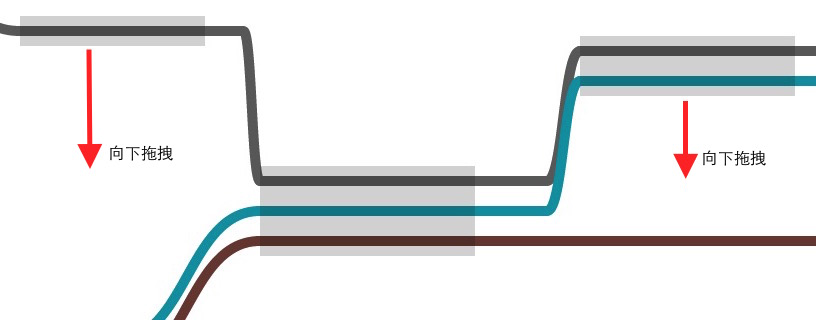
\includegraphics[width=0.4\textwidth, fbox]{alignment-before}
		\label{fig:realignment-before}
	}
	\subfigure[拖拽后]{
		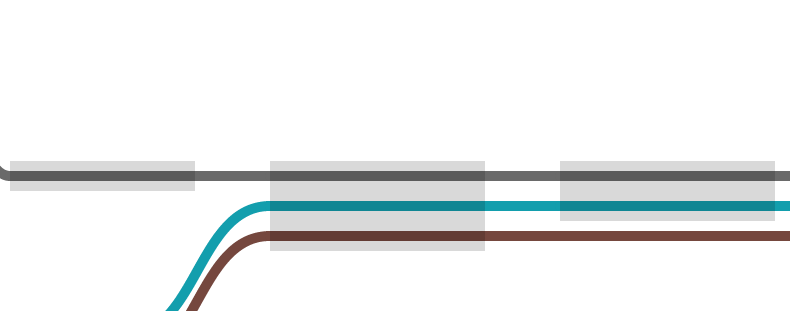
\includegraphics[width=0.4\textwidth, fbox]{alignment-after}
		\label{fig:realignment-after}
	}
	\caption{通过拖拽会话使得线条对齐}
	\label{fig:drag-to-realignment}
\end{figure}
% END == 拖拽会话使对齐

通过手动拖拽可以促使线条重新排序,从而减少线条的交叉,如 Figure \ref{fig:drag-to-reorder} 所示,通过将红色线条的起点拖拽到另外两个线条的小面后,使得线条重新排序,最重减少了两个线条交叉。
% BEGIN == 拖拽会话使得线条重排序
\begin{figure}[htb]
	\centering
	\subfigure[拖拽前]{
		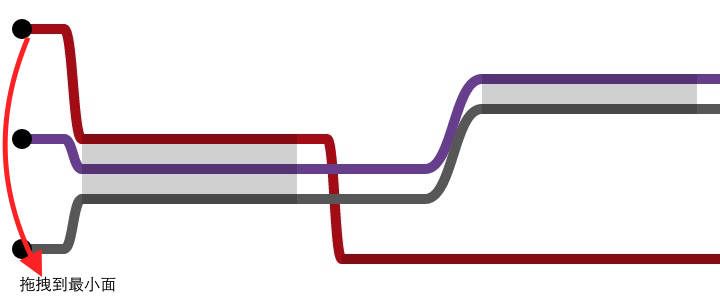
\includegraphics[width=0.4\textwidth, fbox]{order-before}
		\label{fig:order-before}
	}
	\subfigure[拖拽后]{
		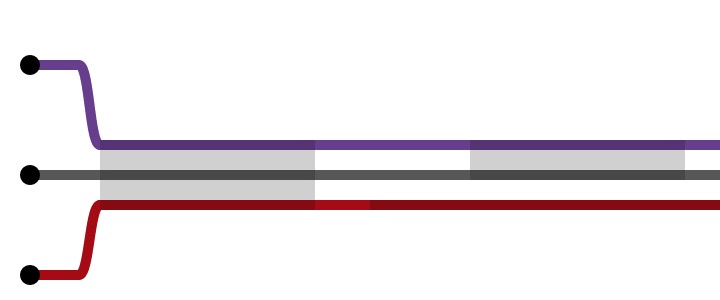
\includegraphics[width=0.4\textwidth, fbox]{order-after}
		\label{fig:order-after}
	}
	\caption{通过拖拽会话使得线条重排序}
	\label{fig:drag-to-reorder}
\end{figure}
% BEGIN == 拖拽会话使得线条重排序

\subsection{隐藏/显示实体}
在生成的storyline中,有时实体数量会比较多,因此线条关系会比较复杂。对于某一个用户而言,它并不需要同时查看所有的实体之间的关系,因此允许用户隐藏他不关心的实体,仅保留它关心的实体显得非常实用。对于隐藏的实体,若用户可以重新勾选使其展现出来。隐藏和显示实体并不影响原始的storyline布局,因此用户可以随意组合自己想要查看的实体,如 Figure \ref{fig:hide-character} 所示。
% BEGIN == 隐藏和显示实体
\begin{figure}[htb]
	\centering
	\subfigure[显示所有实体时]{
		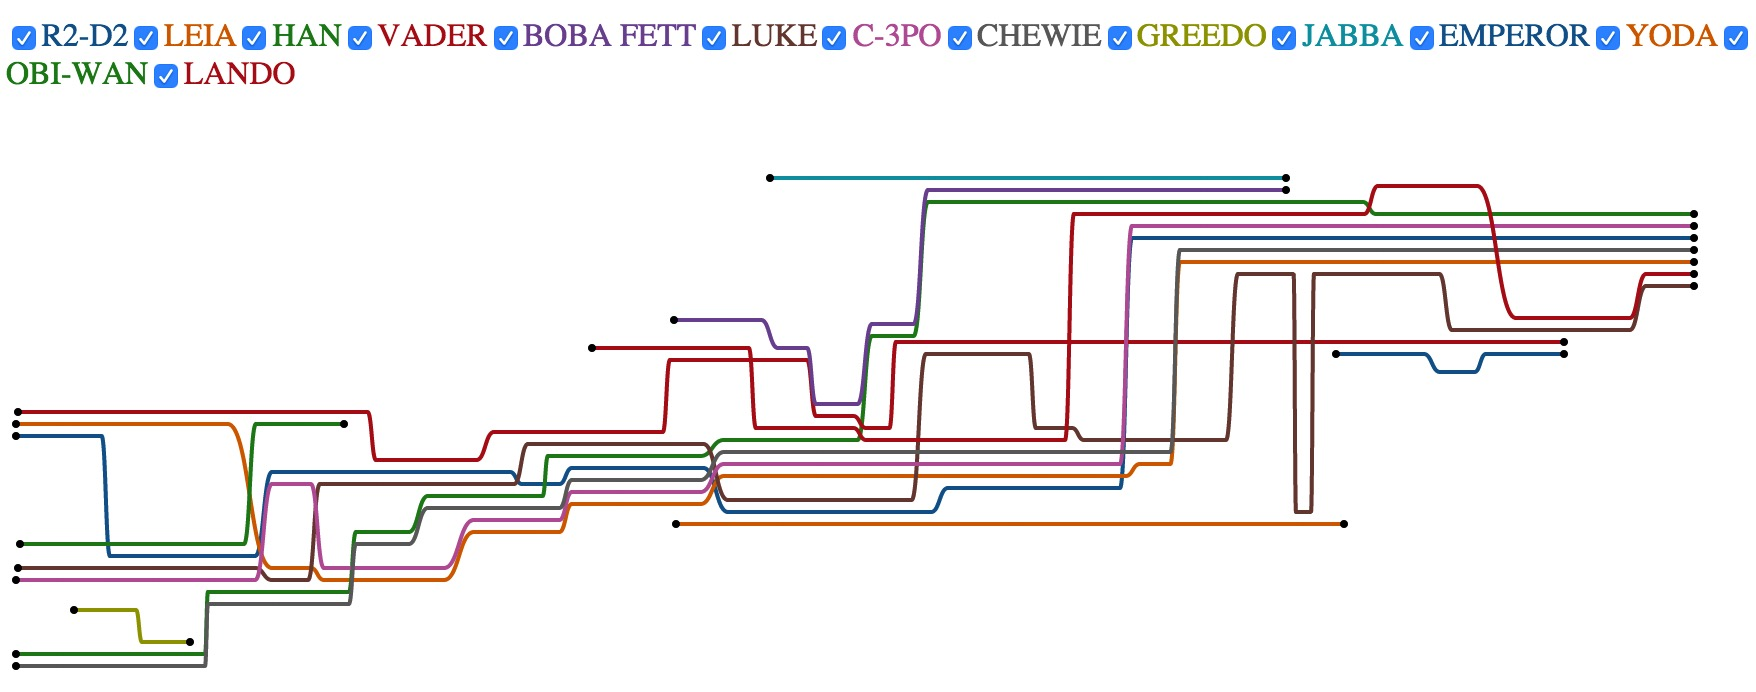
\includegraphics[width=\textwidth, fbox]{hide-character-before}
		\label{fig:hide-character-before}
	}
	\subfigure[隐藏部分实体后]{
		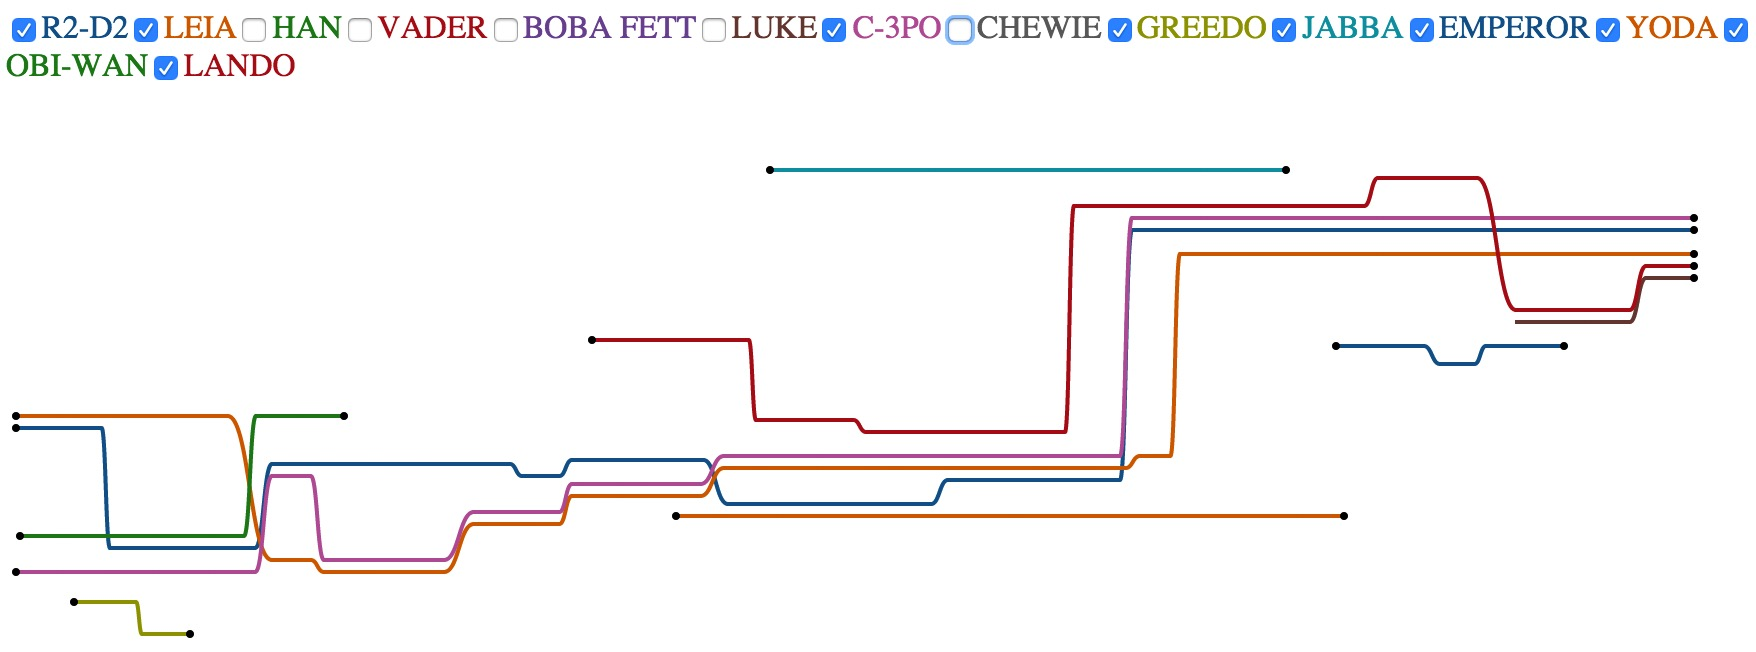
\includegraphics[width=\textwidth, fbox]{hide-character-after}
		\label{fig:hide-character-after}
	}
	\caption{显示和隐藏实体}
	\label{fig:hide-character}
\end{figure}
% BEGIN == 隐藏和显示实体

\subsection{展示会话详情}
通过storyline,用户可以了解哪些实体在什么时间点发生了交互,但是却不知道在该时间点它们之间具体发生了什么事情。为了更好的让用户了解每个会话所发生的事件详情,我们为每个会话都添加了上下文信息。当鼠标移动到会话位置,会出现一个弹框,弹框内包含了该会话的主题,以及与该会话相关的文章的链接地址。用户可以通过主题词了解事件的重要信息,同时还可以点击具体的详情文章了解具体信息,如 Figure \ref{fig:session-with-context} 所示。
% BEGIN == 展示会话详情
\begin{figure}[!htb]
	\centering
		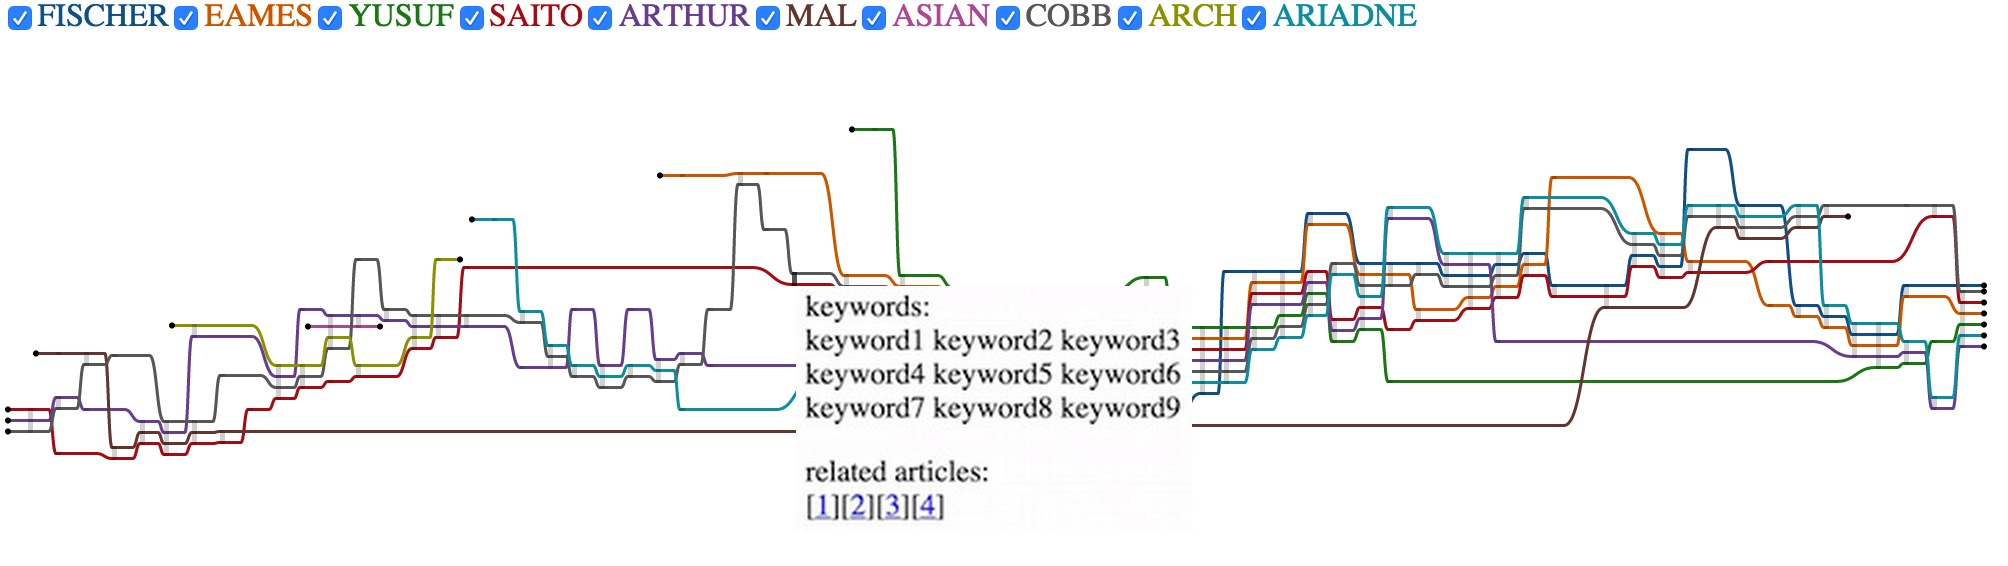
\includegraphics[width=\textwidth, fbox]{session-with-context}
	\caption{显示会话详情}
	\label{fig:session-with-context}
\end{figure}
% END == 展示会话详情

\section{可视化实现}
为了更好的展示可视化结果并提供交互式的用户体验,我们选择了Web端作为展示平台,因此在实现过程中使用的主要技术为JavaScript和SVG,并且使用了d3.js\footnote{http://d3js.org/},Viz.js\footnote{https://github.com/mdaines/viz.js}和Graphlib-dot\footnote{https://github.com/cpettitt/graphlib-dot/wiki}等开源框架来来帮助我们实现绘图以及运行和解析DOT。
\subsection{线条绘制}
在storyline中主要包括两类线段,分别是:会话内部的线段,连接会话的线段。对于会话内部的线段,在绘图是我们只需将其保持水平即可,也就是只需要线段的起点和终点坐标就可以确定。然而对于连接两个会话的线段,如果仅仅是用直线将其连接起来,会使storyline中出现趋多折线,看起来不够平滑。因此连接会话的线段我们需要用曲线去表示,在SVG中可以使用贝塞尔曲线\footnote{http://en.wikipedia.org/wiki/Bezier\_curve}来表示Path。我们采用三次曲线,它由两个端点$a$,$b$以及两个中介点$m1$,$m2$来确定,通过实验分析,我们最终选择了如 Figure \ref{fig:bezier-curve} 所示的中介点来控制曲线。中介点的坐标确定如下:
\begin{subequations}
\begin{align}
	x_{m1} = \frac{1}{2}\left ( x_a + x_b \right ), \quad y_{m1} = y_a \\
	x_{m2} = \frac{1}{2}\left ( x_a + x_b \right ), \quad y_{m2} = y_b
\end{align}
\end{subequations}
为了让连接会话的线段尽可能保持对齐,我们不能简单的将线段的起点和终点作为曲线的两个端点,而应在线段上靠近终点附近开始绘制曲线,而其余部门则保持水平对齐。对于线段$ab$,曲线起点$s$的选取可以根据以下公式:
\begin{equation}
\label{eq:curve-start}
x_s = x_b - Min(panel\_width*10, (x_b - x_a)*3.0/10.0);
\end{equation}
其中$pannel\_width$表示每个单位时间所占的像素长度。从公式 \ref{eq:curve-start} 可以看出,如果线段的起点和终点在水平方向上相距较远,则曲线的起点设置成距离终点10个单位时间的长度;相反如果它们距离很近,则设置为距离终点$3/10$的地方。以上的具体数值是根据实验分析得到的经验值,可以根据实际情况进行调整。
% BEGIN == segment
\begin{figure}[htb]
	\centering
	\subfigure[三次曲线中介点选取]{
		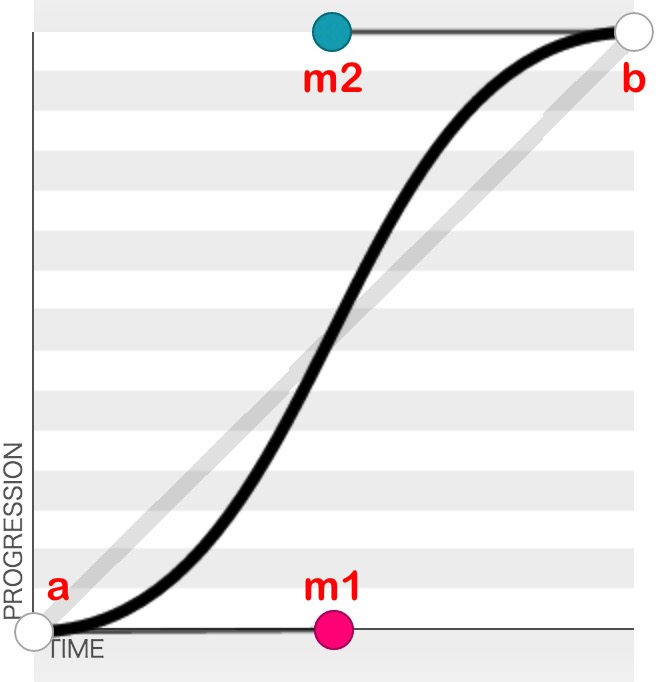
\includegraphics[width=0.27\textwidth]{bezier-curve-sample}
		\label{fig:bezier-curve}
	}
	\subfigure[曲线实例1]{
		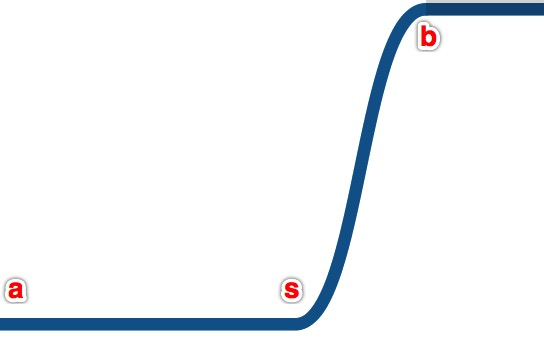
\includegraphics[width=0.45\textwidth]{bezier-curve-instance1}
		\label{fig:bezier-curve-instance1}
	}
	\subfigure[曲线实例2]{
		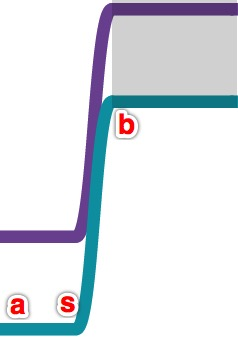
\includegraphics[width=0.19\textwidth]{bezier-curve-instance2}
		\label{fig:bezier-curve-instance2}
	}
	\caption{会话之间的连接线段绘制}
	\label{fig:session-space}
\end{figure}
% END == segment

\section{实验结果与分析}

\subsection{定量分析}
我们首先比较本文方法与TM方法在生成storyline时所消耗的时间,从 Table \ref{table:quantitative-analysis} 可以很清楚的看到,TM方法所消耗的时间是本文方法的百倍以上。原因是TM算法是基于遗传算法进行优化,而遗传算法的问题之一就是它需要设置一个较大的繁衍代数,因此消耗的时间会很长。
\begin{table}[htb]
\caption{本文方法与TM方法的定量对比}
\label{table:quantitative-analysis}
\begin{center}
  \begin{tabular}{|*{9}{l |}}\hline
                    & \multicolumn{2}{c|}{数据源} & \multicolumn{2}{c|}{运行时间(秒)} & \multicolumn{2}{c|}{线条交叉数} & \multicolumn{2}{c|}{线条摆动数目} \\ \hline
                    & 实体数目 &  时间片数 & 本文方法 & TM 方法 & 本文方法 & TM 方法 & 本文方法 & TM 方法 \\ \hline
    StarWars & 14           & 50             & 3              & 130       &  48          &  93         &  66           & 133        \\ \hline
    Inception &  8            & 71             & 3              & 150       &  49          &  99         &  82           & 162        \\ \hline
    Matrix      & 14           & 42             & NaN         & 172       &  NaN       &  43         &  NaN       & 94          \\ \hline
  \end{tabular}
\end{center}
\end{table}

% BEGIN == segment
\begin{figure}[htb]
	\centering
	\subfigure[StarWars]{
		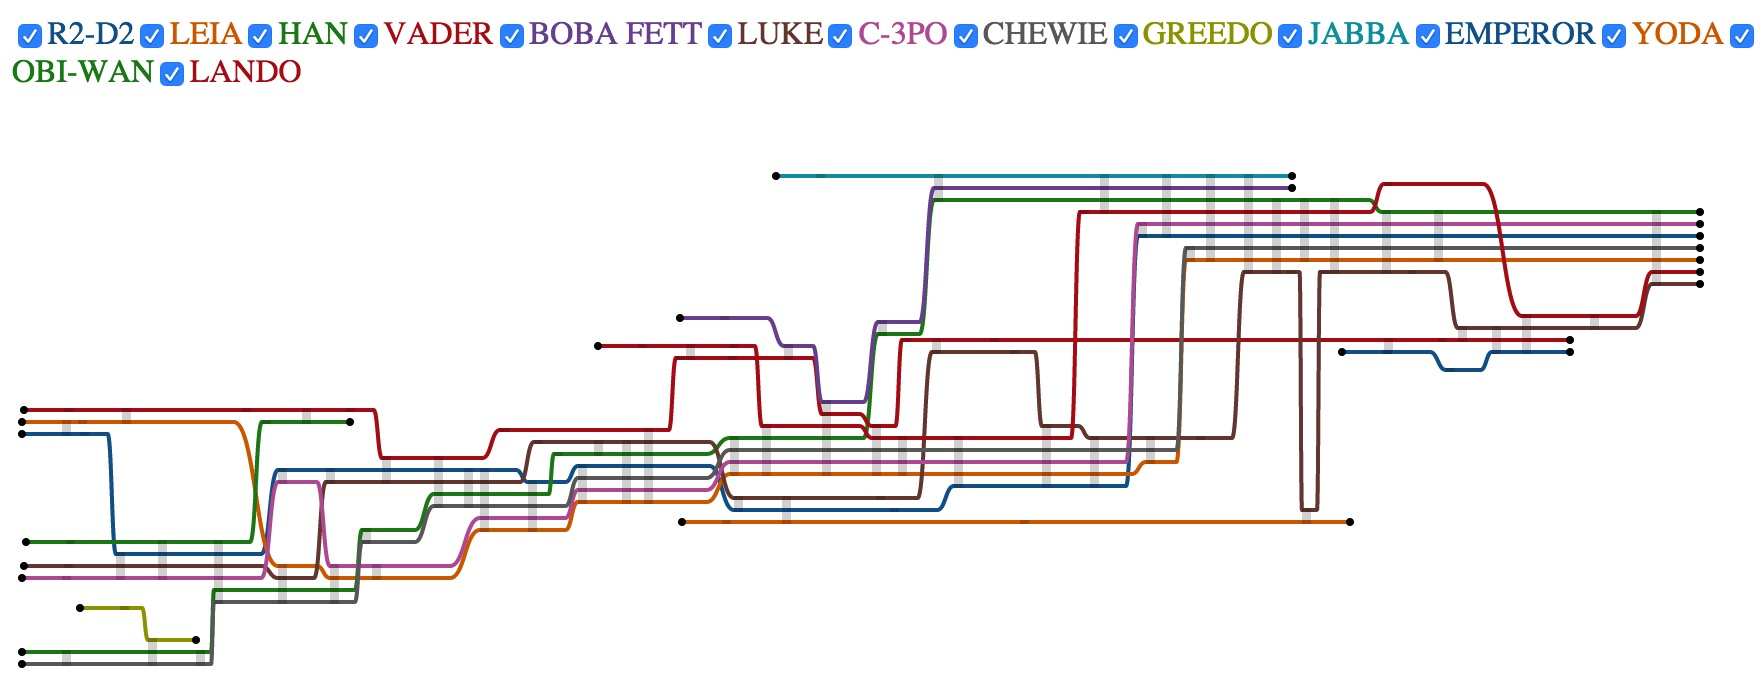
\includegraphics[width=\textwidth, fbox]{layout-starwars}
		\label{fig:star-wars}
	}
	\subfigure[Inception]{
		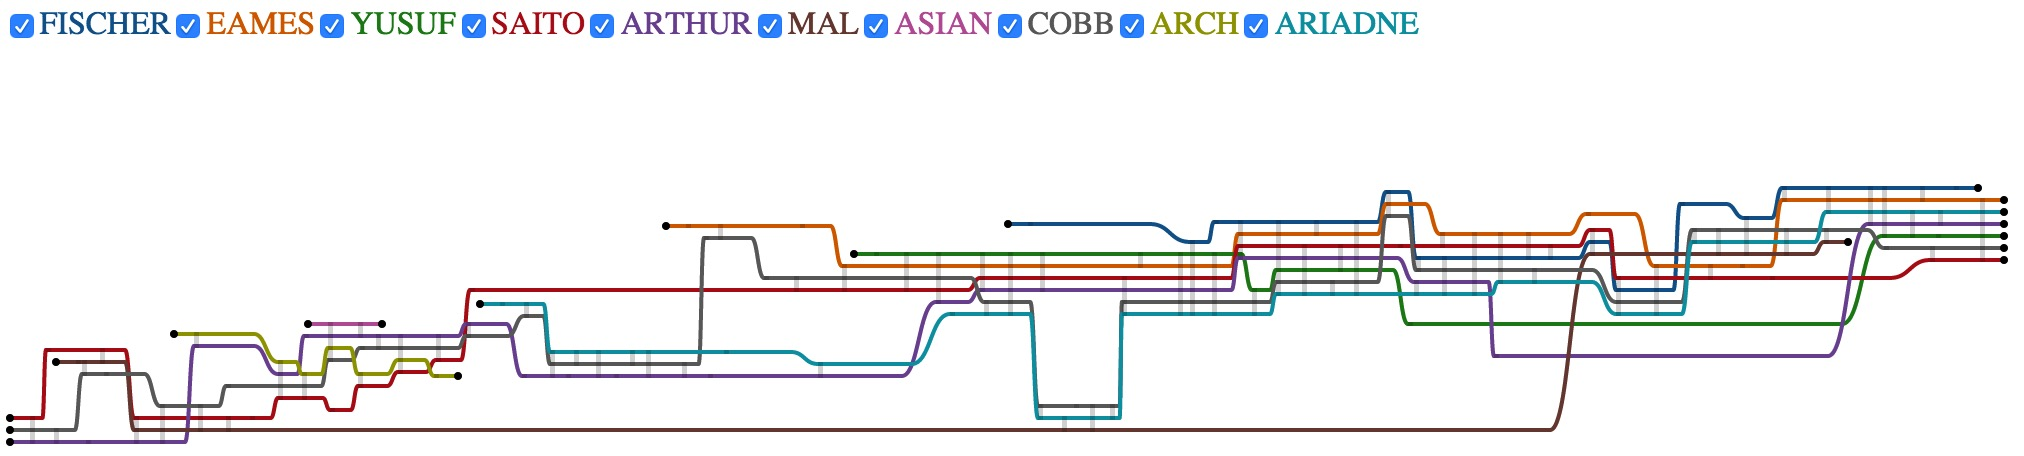
\includegraphics[width=\textwidth, fbox]{layout-inception}
		\label{fig:inception}
	}
	\subfigure[Matrix]{
		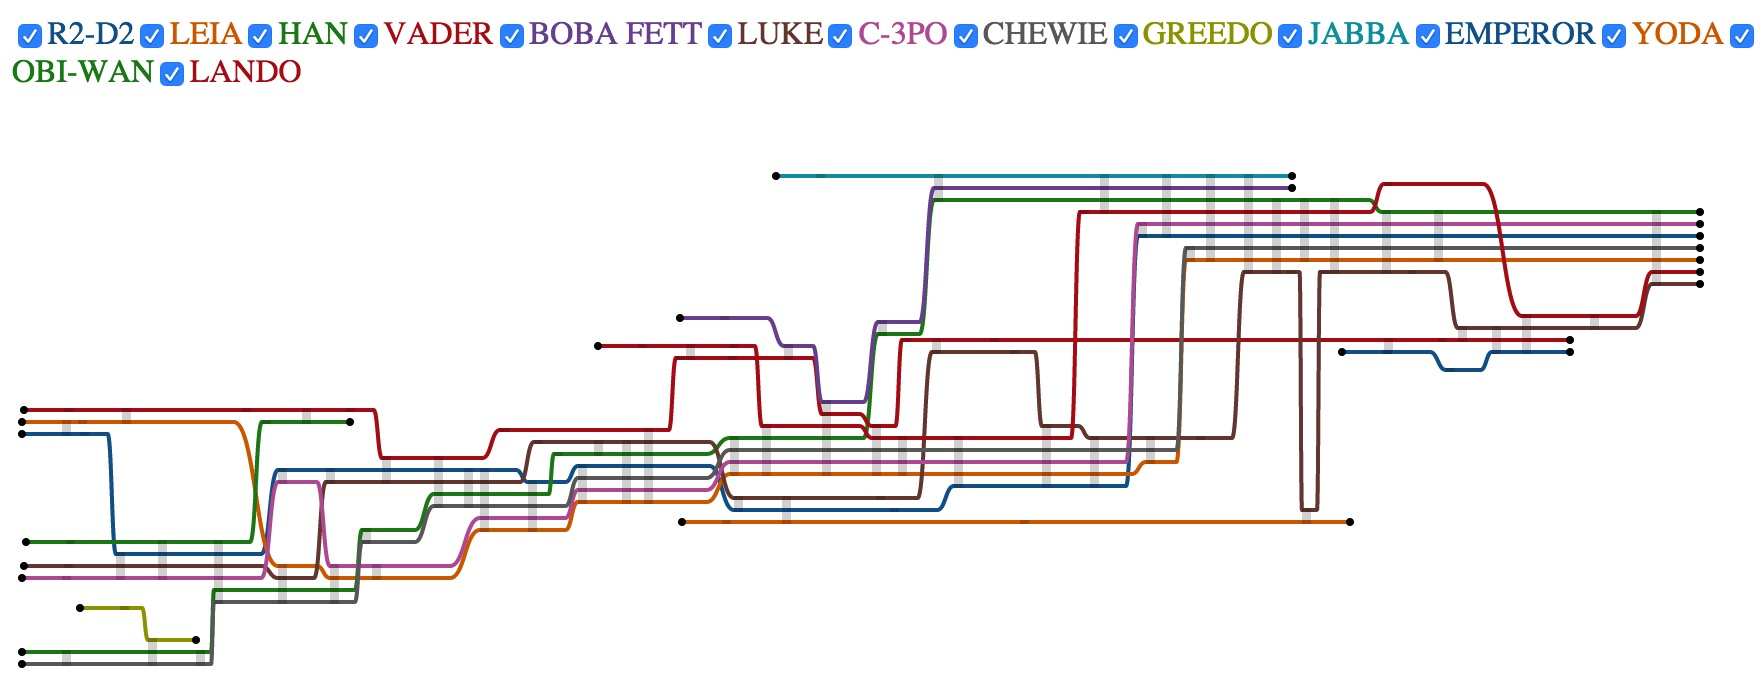
\includegraphics[width=\textwidth, fbox]{layout-starwars}
		\label{fig:matrix}
	}
	\caption{最终结果}
	\label{fig:layout-sample}
\end{figure}
% END == segment

\subsection{案例分析}
新闻故事的人物关系 storyline,以“Edward Snow”事件为例。

\section{本章小结}
本章我们首先介绍了一种可视化方法-storyline,该方法是用于描述实体之间随时间变化的交互关系。然而已有的生成storyline 的方法中,有些是针对特定领域的,有些是计算过程非常耗时的,有些需要纯手动绘制。为了能运用storyline来描述新闻事件中人物之间的交互关系,我们提出了自己的一套方法来生成storyline。该方法分三个步骤:排序,对齐,压缩。每一步分别对storyline的一个指标进行优化,通过迭代的方法最终获得一个最优的图形。最后,我们还根据storyline的特点提供了几种用户交互方式,既可以进一步优化图形,还可以让用户更好的理解事件详情。

